% -*- mode: LaTeX -*-
%%

%%%%%%%%%%%%%%%%%%%%%%%%%%%%%%%%%%%%%%%%%%%%%%%%%%%%%%%%%%%%%%%%%%%%%%%%%%%%%%%

\section{Results and Discussion}
\label{sec:evaluation}

\begin{figure}
  \centering
  \includegraphics[width=0.9\columnwidth]{3561} 
  \caption{Run 1. Used 3561 MHz frequency}
  \label{fig:3561}
\end{figure}

After the 4 measurement runs completed on Shout, we perform an analysis with the SPLAT! tool using the same frequencies, radio
locations and following the same method discussed in section 3. We convert the acquired data to Excel spreadsheets that are later
imported into RStudio to create our plots. Each dot on the plot is a pairwise connection between the transmitter and receiver at the 
given frequency. Due to the multitude of dots we neglect from naming each dot as it overwhelms the plot for further analysis. Due to the unknown
reference for either Shout or SPLAT! we are unable to directly compare the two. However, we will compare the two using the path loss 
exponent which happens to be the slope of the linear regression line. Following the path loss exponent analysis we will do a brief terrain 
analysis of the results to verify if what we got appears to be accurate. 

\begin{table}[h!]
\centering
\begin{tabular}{||c c c c||} 
 \hline
 \textbf{Run \#} & \textbf{Frequency} & \textbf{Shout} & \textbf{SPLAT!} \\ [0.5ex] 
 \hline\hline
Run 1 & 3561 MHz & -0.0086 & -0.0154 \\ 
Run 2 & 2620 MHz & -0.0114 & -0.0186 \\ 
Run 3 & 3550 MHz & -0.0132 & -0.0113 \\ 
Run 4 & 3690 MHz & -0.0163 & -0.0103 \\ [1ex] 
 \hline
\end{tabular}
\caption{Path Loss Exponents for each run.}
\label{table:1}
\end{table}

\subsection*{Path Loss Exponent}
Due to the POWDER platforms uncalibrated radios there is not a single reference point for the Shout data. This is the reason why all of our plots for each
run define the Y-axis as the received power in dBm with an unknown reference. Notice that SPLAT!'s data is represented by the red color
while Shout's data is represented by the blue color. Table~\ref{table:1} summarizes the path loss exponents for each run.

Run 1 (Figure~\ref{fig:3561}), was conducted on the 3561 MHz frequency in early October at around 11AM. This run followed the typical round-robin fashion, 
where each circle on the plot represents a pairwise connection between the transmitter and receiver. The slope for Shout in run 1 was 
$-0.00862$, this tells us that the power decays proportionally to $d^{-0.00862}$ where $d$ is the path length. Similarly, we determined the
measurements fit of SPLAT!. The path loss exponent is $-0.0154$ that is the power decays proportionally to $d^{-0.0154}$. We can see 
SPLAT!'s path loss exponent has a steeper slope. That is for the 3561 MHz frequency, SPLAT! has over-predicted the path loss when 
compared to Shout's ground truth measurements. 

\begin{figure}
  \centering
  \includegraphics[width=0.9\columnwidth]{2620}
  \caption{Run 2. Used 2620 MHz frequency}
  \label{fig:2620}
\end{figure}

We now conduct a similar procedure to the remaining runs. Run 2 (Figure~\ref{fig:2620}) was conducted in early November at around 9AM and used the
largest amount of nodes within our experiments. Shout's path loss exponent was $-0.0114$ with a power decay proportional to $d^{-0.0114}$. 
While SPLAT!'s path loss exponent was $-0.0186$ with a power decay proportional to $d^{-0.0186}$. These are fairly close but once again
SPLAT! is over-predicting the POWDER platform's radio path loss at the 2620 MHz frequency. 

Run 3 (Figure~\ref{fig:3550}) and run 4 (Figure~\ref{fig:3690}) were conducted in late November. Specifically, run 3 was conducted at around
2AM while run 4 occurred around 6AM. For run 3, Shout's path loss exponent is $-0.0132$ while SPLAT!'s is $-0.0113$. Run 3 offers the 
closest in comparing the path loss exponent values for the data collected. However, this time SPLAT! is under-predicting the POWDER platforms
path loss for the 3550 MHz frequency. Similarly, in run 4 we see SPLAT! under-predicting the path loss on the 3690 MHz 
frequency. In run 4 we see that Shout's path loss exponent is $-0.0163$, while SPLAT!'s path loss exponent is $-0.0103$. 
 
 \begin{figure}
  \centering
  \includegraphics[width=0.9\columnwidth]{3550}
  \caption{Run 3. Used 3550 MHz frequency}
  \label{fig:3550}
\end{figure}

\subsection*{Terrain Analysis}
The purpose of this section is to bring SPLAT! to real life and compare the model to physical locations. We will be utilizing Google Maps
to take a closer view of the environment in run 1. Notice that in figure~\ref{fig:3561}, we label the best and worst path loss nodes for each
data set. We will focus on the two nodes with the best path loss, and the two nodes with the worst path loss and compare Shout and SPLAT!
when differences arise. 

\subsubsection*{Best Path Loss}
We first look at the two nodes in run 1 with the best path loss. Table~\ref{table:2} lists the best path loss nodes for both Shout and SPLAT!,
at the 3561 MHz frequency. We can see that for both data sets, MEB and Browning hold the best propagation values. 
Figure~\ref{fig:mebBrown} shows the Google Maps image of the two nodes. Both nodes are rooftop base stations with an open Line of Sight.
We believe that these two nodes received the best propagation simply due to the distance between them and the fact that there is nothing
directly blocking them.  

\begin{figure}
  \centering
  \includegraphics[width=0.9\columnwidth]{3690}
  \caption{Run 4. Used 3690 MHz frequency}
  \label{fig:3690}
\end{figure}

\begin{table}[h!]
\centering
\begin{tabular}{||c c c||} 
 \hline
 \textbf{Set} & \textbf{Nodes} & \textbf{Received Power} \\ [0.5ex] 
 \hline\hline
Shout & MEB, Browning  & -52 dBm \\ 
SPLAT! & MEB, Browning  & -83 dBm \\ [1ex] 
 \hline
\end{tabular}
\caption{Run 1, best path loss for Shout and SPLAT!.}
\label{table:2}
\end{table}

\begin{table}[h!]
\centering
\begin{tabular}{||c c c||} 
 \hline
 \textbf{Set} & \textbf{Nodes} & \textbf{Received Power} \\ [0.5ex] 
 \hline\hline
 Shout & MEB, SMT & -87 dBm\\ 
 SPLAT! & MEB, Sagepoint & -115 dBm\\ [1ex] 
 \hline
\end{tabular}
\caption{Run 1, worst path loss for Shout and SPLAT!.}
\label{table:3}
\end{table}

\begin{figure}
  \centering
  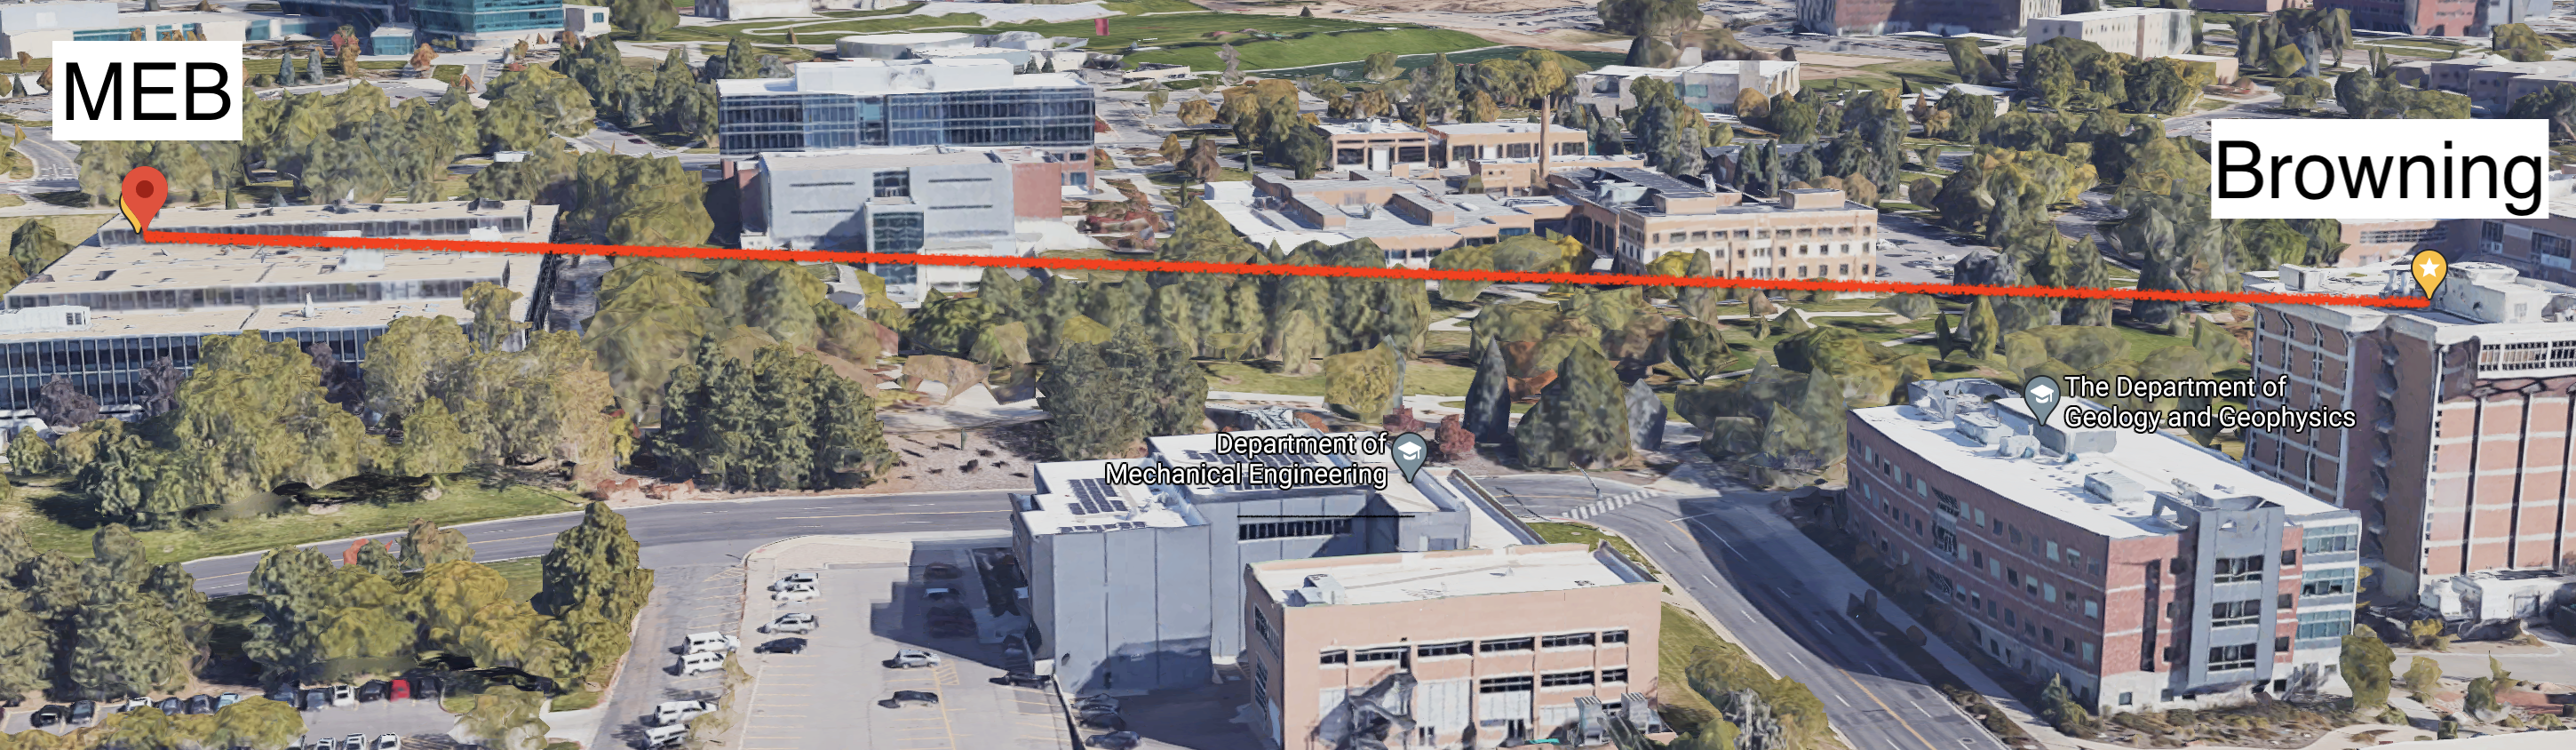
\includegraphics[width=0.9\columnwidth]{mebBrown}
  \caption{MEB left and Browning right}
  \label{fig:mebBrown}
\end{figure}

\subsubsection*{Worst Path Loss}
We now look at the two worst nodes with regards to propagation loss. Table~\ref{table:3} lists the worst path loss nodes for both Shout and SPLAT!
at the 3561 MHz frequency. For SPLAT! these two nodes are MEB and Sagepoint. We note that Sagepoint is the only fixed endpoint node for run 1
and is 1.5 meters above the ground, while MEB is a rooftop base station. From figure~\ref{fig:worst} we notice that the environment between MEB 
and Sagepoint is not a clear line of sight. In fact, three sports fields, the student life center, a traffic induced road, and multiple housing units lie 
in-between these two nodes. Furthermore, since Sagepoint is a fixed endpoint node it is placed behind a wall that is not facing the MEB. 

However, Shout thinks differently. It believes that the two worst nodes are MEB, and South Medical Tower (SMT).
The environment between these two include the Biotechnology Building, a traffic induced road, parking structures, and the College of Pharmacy.
However, both MEB and SMT are rooftop base stations with MEB being the shorter one. 

\subsection*{Discussion}
We now offer a few insights as to why we got the results we did. We can see how early hours affected Shout's data in run 3. In figure~\ref{fig:3550}
where we can see that at a striking distance of about 2128 meters we appear to be getting $-78$ dBm in received power compared to SPLAT!'s
$-104$ dBm, for the Friendship Manor and SMT nodes. Again we can't compare point-to-point due to unknown reference, but it is a bit of an astonishment
when compared to the rest of Shout's data where about half the points are underneath $-78$ dBm given their respective smaller path length.

As expected for all case in every run we saw multipath powers with exponentially decreasing magnitude as a function of distance. Meaning
that in all cases we saw propagation loss increase with distance. As discussed in section 2, there exists multiple path loss models that can be
used depending on the parameters available to us. For example, SPLAT! follows the Longley-Rice path loss model, it just could so happen that
this model is simply not intended for the Utah environment on a campus with a dense city-like section. 

Differences between the ground truth and modeling tools will always occur. Again this is due to time, weather, un-updated map data for the modeling 
tool, or simply the wrong model is being used. During this 8 week project we saw the seasons transform from summer to fall. That is measurements
taken at different time periods will have an affect on our data. A good exercise would be to continue this work using different frequency bands, POWDER
nodes, and path loss models. 

%%%%%%%%%%%%%%%%%%%%%%%%%%%%%%%%%%%%%%%%%%%%%%%%%%%%%%%%%%%%%%%%%%%%%%%%%%%%%%%

%% End of file.
